% Anexo: Manual de Operador para Captura de Datos de Entrenamiento
\chapter*{Anexo I: Manual de Operador para Captura de Datos de Entrenamiento}
\addcontentsline{toc}{chapter}{Anexo I: Manual de Operador para Captura de Datos de Entrenamiento}

Este anexo es un manual detallado para la captura de datos de entrenamiento usando la aplicación gráfica Neural Analytics Capturer. Explica cada pantalla y el flujo de trabajo para que cualquier persona pueda completar el proceso correctamente.

Esta es una aplicación de terminal que permite capturar datos de EEG desde el dispositivo BrainBit. El objetivo es registrar la actividad cerebral mientras el usuario piensa en diferentes colores (rojo, verde, etc.) para entrenar un modelo de IA que pueda reconocer estos patrones.

\section*{1. Antes de empezar}
\begin{itemize}
    \item Asegúrese de que el dispositivo BrainBit está cargado y listo.
    \item Compruebe que la aplicación Neural Analytics Capturer está instalada y abierta en el ordenador.
    \item Verifique que el dispositivo está conectado correctamente (por Bluetooth o cable).
\end{itemize}

Es importante también hacer un plan de que datos se quieren capturar, es decir, qué tipo de actividad mental se va a registrar (pensar en rojo, verde, etc.). Y sobretodo, en que lugares se va a realizar la captura, ya que el entorno puede influir en la calidad de la señal.

Esto último es importante, ya que la varianza de datos es critica para poder eliminar cualquier tipo de sesgo en el modelo. Por ejemplo, si se quiere capturar datos mientras se piensa en rojo, es recomendable hacer una muestra en un lugar tranquilo y otro en un lugar con ruido ambiental, para que el modelo aprenda a distinguir entre ambos contextos.

\newpage
\section*{2. Verificación de impedancia y calidad de señal}
Una vez seleccionado el dispositivo, la aplicación mostrará el estado de los electrodos (T3, T4, O1, O2). Si algún electrodo aparece en rojo o con un símbolo de error, ajuste su posición hasta que todos estén en verde o correcto. No continúe hasta que la calidad sea adecuada.

\begin{figure}[h!]
    \centering
    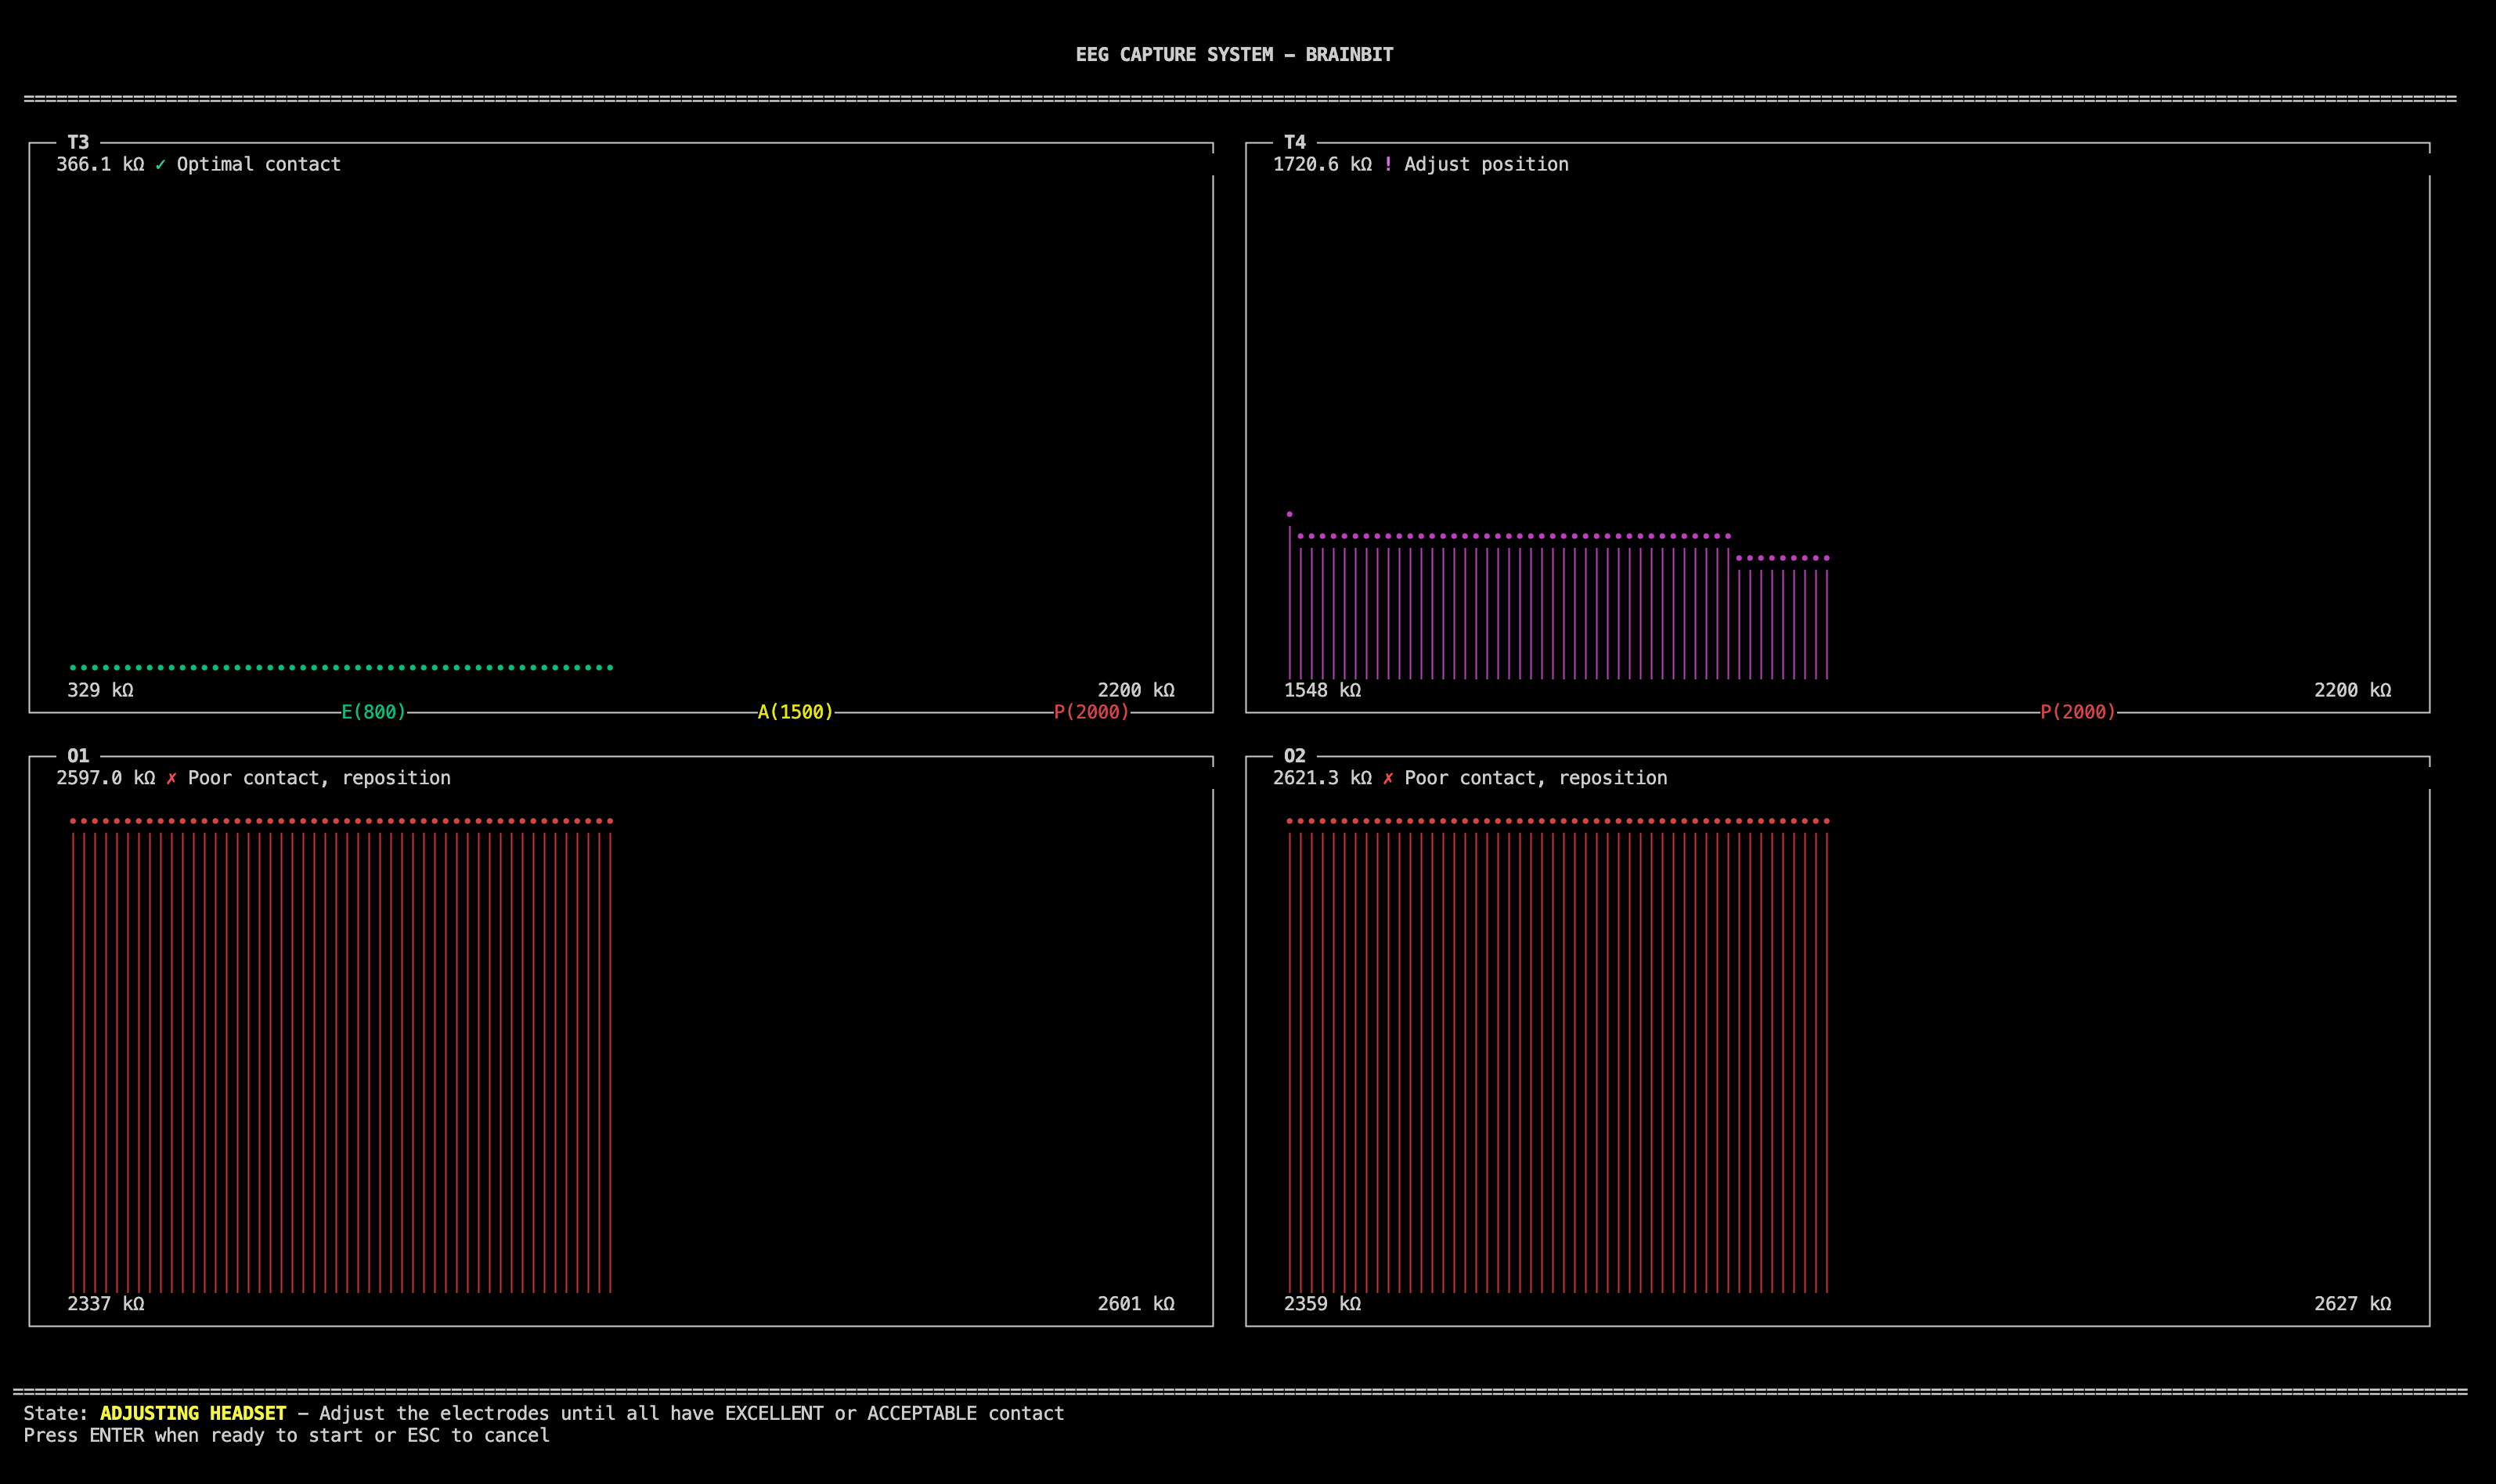
\includegraphics[width=0.8\textwidth]{assets/screenshots/capturer/impedance_check.png}
    \caption{Verificación de impedancia y calidad de señal.}
\end{figure}

Una vez que todos los electrodos estén en verde, pulse el botón \textbf{Comprobar Impedancia} para confirmar que la señal es adecuada. Si hay algún problema, ajuste los electrodos y repita la comprobación.

\newpage
\section*{3. Inicio y monitorización de la captura}
Pulse el botón \textbf{Iniciar Captura} para comenzar. En pantalla verá gráficas en tiempo real de la señal de cada electrodo. No es necesario interpretar los gráficos, solo asegúrese de que se están moviendo y no hay mensajes de error.

\begin{figure}[h!]
    \centering
    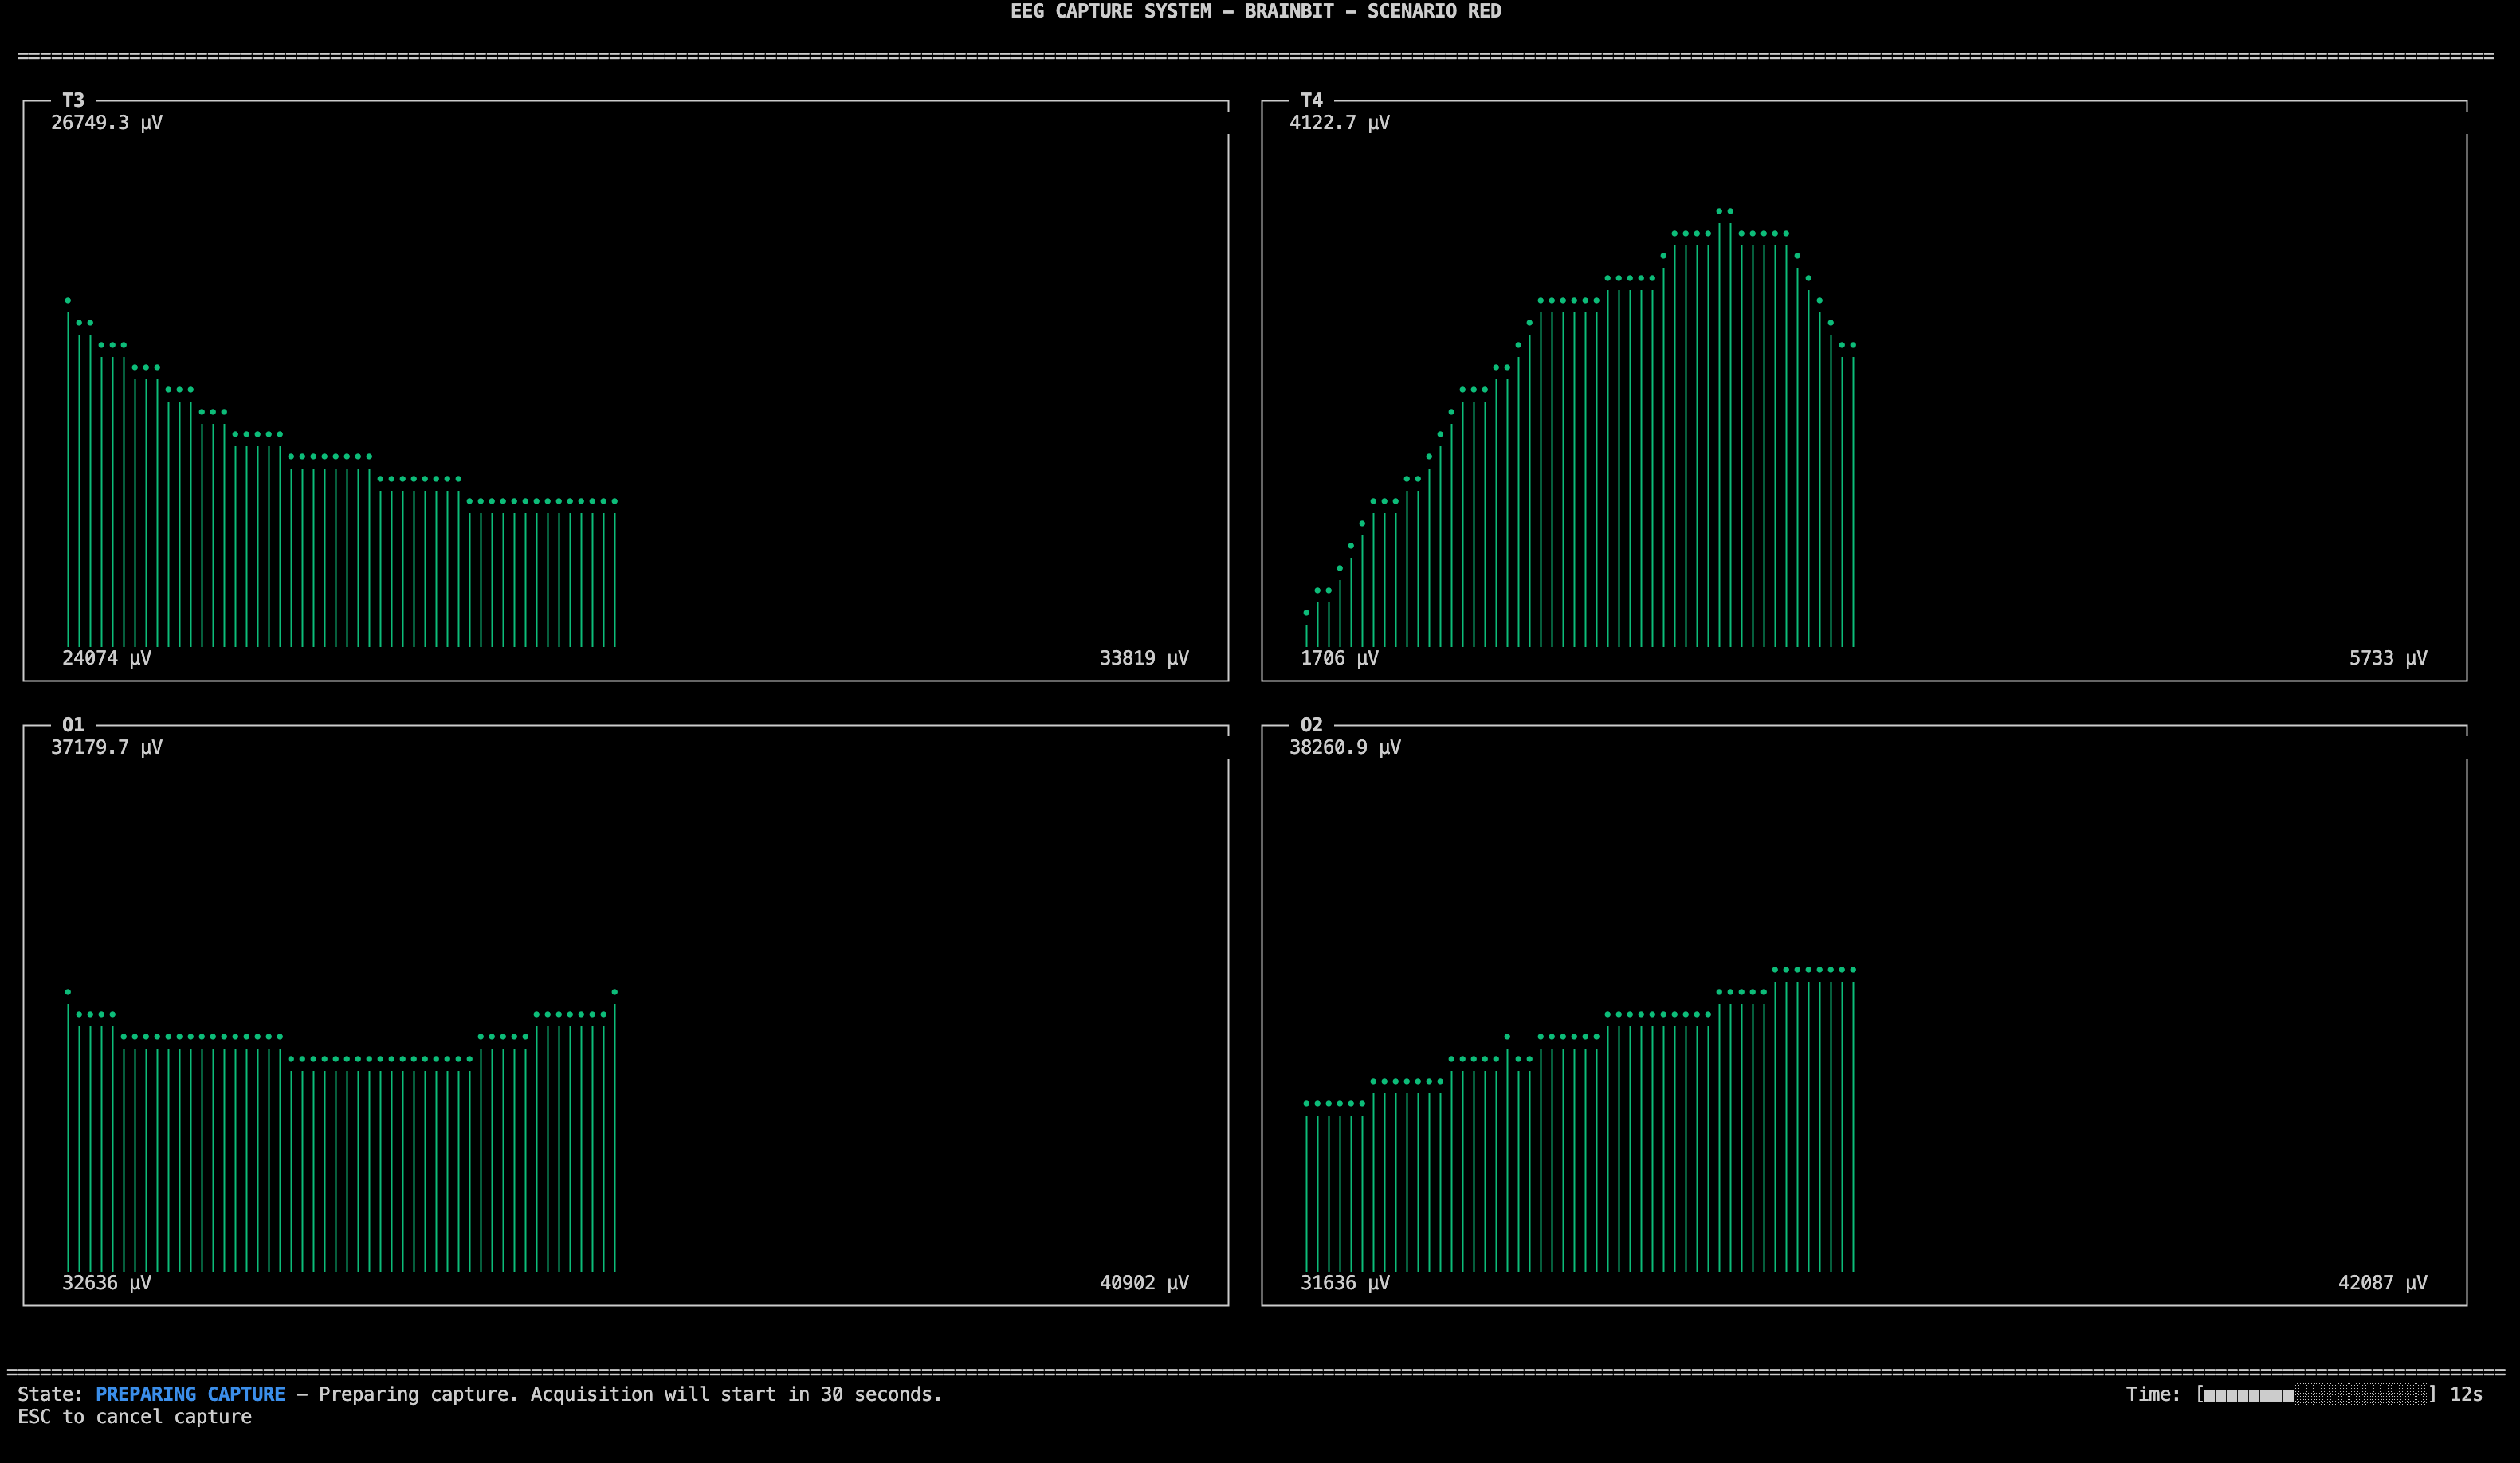
\includegraphics[width=0.8\textwidth]{assets/screenshots/capturer/data_acquisition.png}
    \caption{Adquisición de datos en tiempo real.}
\end{figure}

\section*{4. Finalización y guardado de datos}
Cuando termine la sesión, se escuchará un mensaje de voz indicando que la captura ha finalizado, y acto seguido, la captura se detendrá automáticamente. Los nuevos datos se guardarán en un archivo CSV en la carpeta \texttt{data/} del proyecto. Asegúrese de que el archivo se ha creado correctamente.

\section*{5. Mensajes y advertencias}
\begin{itemize}
    \item Si algún electrodo pierde contacto, la aplicación lo indicará y deberá ajustarlo antes de continuar.
    \item Si la señal es débil, aparecerá un aviso. Siga las recomendaciones en pantalla.
    \item Si ocurre un error grave, cierre y vuelva a abrir la aplicación.
\end{itemize}

\section*{6. Consejos prácticos}
\begin{itemize}
    \item Coloque los electrodos con cuidado y evite que se muevan durante la sesión.
    \item No cierre la aplicación ni apague el ordenador hasta que vea el mensaje de que los datos se han guardado correctamente.
    \item Si tiene dudas, consulte este manual o pida ayuda al responsable.
\end{itemize}
